\documentclass[a4paper]{article}

\usepackage[utf8]{inputenc}
\usepackage[T1]{fontenc}
\usepackage{textcomp}
\usepackage[italian]{babel}
\usepackage{graphicx}
\usepackage{siunitx}
\usepackage{hyperref}
\usepackage{float}
\usepackage{amsmath, amssymb}

\sisetup{uncertainty-mode=separate}

\title{Relazione di Laboratorio 3 - Caduta}
\author{Walhout Francesco - Iallorenzi Michele}

\begin{document}
    \maketitle

    \section{Introduzione}
    Un oggetto soggetto ad un accelerazione costante $g$ che si muove con una velocità
    iniziale $v_0$ partendo dalla posizione $h_0$ obbedisce alla seguente legge oraria:
    \begin{equation}
        h(t)= \frac{1}{2}gt^2+v_0t+h_0 \label{eq:legge_oraria}
    \end{equation}
    Ignorando l'attrito dell'aria e la variazione della forza di gravità, l'altitudine di
    un oggetto in caduta libera in prossimità della superficie terrestre segue questa legge.
    Vogliamo quindi testare la validità di questa approssimazione misurando l'altezza dal
    suolo di un grave in caduta libera, ottenuta analizzando una registrazione video.
    \subsection{Strumenti utilizzati}
    \begin{itemize}
        \item Un grave.
        \item Uno smartphone o videocamera.
        \item Un metro a nastro.
    \end{itemize}

    \section{Misure ed Analisi}
    \subsection{Preparazione}
    Per poter misurare l'altezza del grave (nel nostro caso una pallina) osservando una registrazione dello stesso
        è necessario porre un metro a nastro in modo che il grave possa caderci accanto;
        inoltre è opportuno che il dispositivo di registrazione punti direttamente
        all'esperimento, in modo da non distorcere l'immagine per gli effetti di prospettiva.
        Il grave è stato fatto cadere da un altezza di circa $\SI{2}{\m}$, ma il valore
        preciso dell'altezza iniziale non è rilevante, né è rilevante se il peso è stato
        lasciato cadere da fermo o se ha subito una spinta durante il rilascio: infatti
        possiamo iniziare a prendere misure della sua posizione in qualsiasi punto della
        registrazione, scegliendo l'istante iniziale $t=0$, e quindi l'altezza e la
        velocità iniziale, arbitrariamente.\\
        La fotocamera che abbiamo utilizzato ha registrato a $120$ frame al secondo, 
        restituendo un video di $30$ frame al secondo, rallentato quindi di $4$ volte,
        permettendo così di campionare più punti nel breve periodo di caduta.\\
        Un fotogramma della registrazione ottenuta è mostrato in figura \ref{fig:fotogramma}.
        \begin{figure}[ht!]
            \centering
            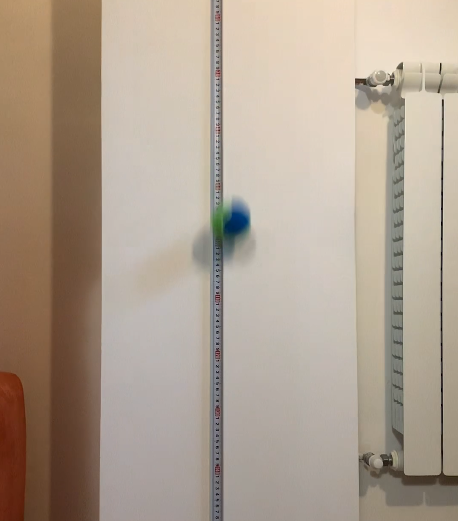
\includegraphics[width=0.8\textwidth]{extra/fotogramma.png}
            \caption{Un fotogramma della registrazione del grave in caduta libera.
            Si noti la sfocatura dovuta al movimento che abbiamo supposto essere la
            principale causa di errore di misura.}
            \label{fig:fotogramma}
        \end{figure}
    \subsection{Misurazione}
        Per misurare le altezze abbiamo aperto il file della registrazione con un programma
        di editing; dato che le tacche sul metro a nastro risultavano illeggbili per la
        risoluzione insufficiente della registrazione, i dati sono stati presi nelle
        "screen coordinates" fornite dal programma di editing, e poi convertiti in metri
        utilizzando la lunghezza conosciuta del metro a nastro per determinare il rapporto
        di conversione. L'origine è stata posta nell'ultima posizione registrata del peso,
        prima dell'impatto col suolo, i tempi invece sono stati ottenuti moltiplicando
        il numero di frame trascorsi dal primo istante campionato per $\frac{1}{120}\si{\s}$,
        ovvero l'inverso del framerate.\\
        Nel video la pallina risulta sfocata dato che vediamo il sovrapporsi delle posizioni
        occupate da essa durante il tempo di esposizione della videocamera, abbiamo
        quindi misurato metà dell'ampiezza di questo spostamento, ovvero metà dell'alone
        sfocato visibile attorno al peso in movimento, e dopo averlo diviso per $\sqrt{12}$ 
        (sotto l'ipotesi che l'errore causato da questo spostamento si distribuisca
        uniformemente) lo abbiamo utilizzato come incertezza di misura, risulta quindi 
        $\sigma_h=0.003m$
    \subsection{Elaborazione dei dati}
    Abbiamo eseguito il fit dei dati secondo l'equazione \ref{eq:legge_oraria} utilizzando
    la funzione curve\_fit della libreria scipy; per il parametro $h_0$ è stata utilizzata
    l'altezza misurata per il primo istante di caduta, quindi il fit ha ottimizzato solo
    i parametri $g$ e $v_0$. I dati sovrapposti al fit ottenuto sono mostrati in figura
    \ref{fig:altezza}.\\
    I valori che il fit restituisce per i parametri sono $v_0=\SI{-3.15\pm 0.01}{\m\per\s}$
    e $g=\SI{-11.5\pm 0.1}{\m\per\s^2}$
    \begin{figure}[ht!]
        \centering
        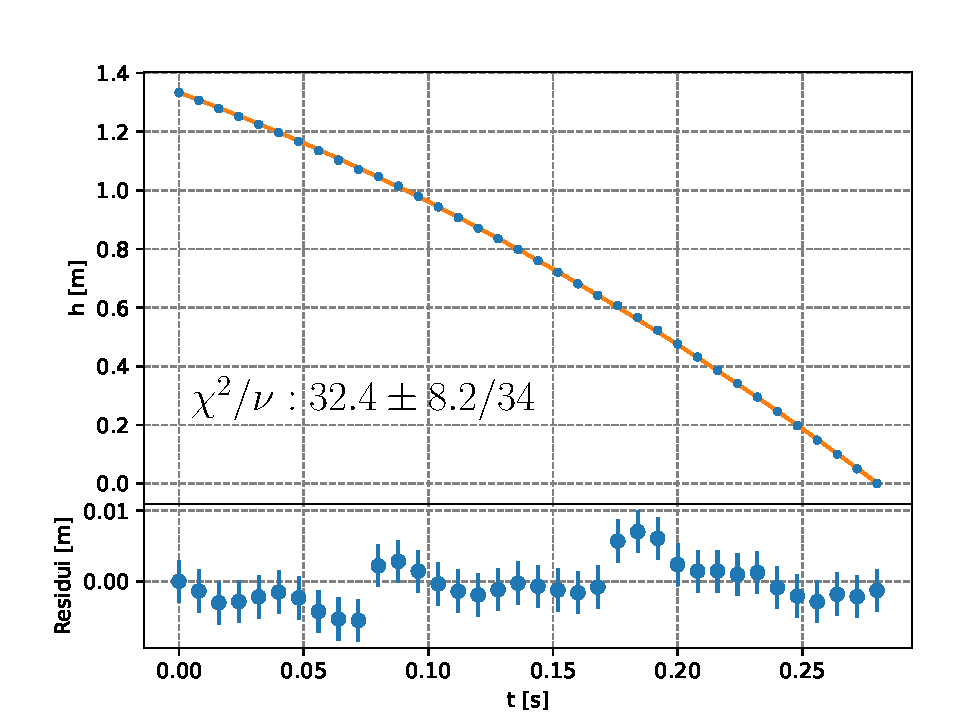
\includegraphics[width=0.8\textwidth]{extra//altezza.pdf}
        \caption{Altezza del grave in funzione del tempo.}
        \label{fig:altezza}
    \end{figure}
    \section{Conclusioni}
    Osservando il grafico dei residui è evidente che il fit sia soddisfacente e che
    quindi gli errori commessi dal trascurare la forza di attrito e altre possibili
    pertubazioni sono trascurabili, tuttavia il valore ottenuto dal fit per l'accelerazione
    di gravità non è compatibile con quello conosciuto di circa $\SI{-9.8}{\m\per\s^2}$.
    Questo errore non è attribuibile all'attrito con l'aria, che porterebbe a misurare un
    accelerazione assoluta minore, altre possibili cause di errore sistematico sono 
    il framerate di registrazione della telecamera il quale potrebbe essere diverso da quello
    riportato oppure gli effetti di prospettiva che possono aver distorto il metro
    utilizzato come riferimento o ingrandito il peso che si trovava più vicino alla
    telecamera rispetto a quest'ultimo.
\end{document}
